\section{Example}
\label{sec:example}

We next present major steps in our approach for detecting the behavioral differences of mapped API elements. In particular, we use JLCA translation tool as an example translation tool, and the \CodeIn{java.io.BufferedInputStream} class in Java as an example API element. TeMAPI extracts mapping relations of API elements defined in JLCA, and generates test cases for each API element in one language and translates those test cases into the other language to detect behavioral differences. TeMAPI includes two major techniques for testing single API classes and multiple API classes.

%----------------------------------------------------
\textbf{Testing Single API Classes.} To test single API class, TeMAPI leverages a state-of-the-art test-generation tool, called Pex~\cite{tillmann2008pex}. Since Pex generates test cases for C\# code, TeMAPI generates test inputs and outputs on C\# code and translates them to Java. We next describe these steps in detail.

As described by its documentation\footnote{\url{http://tinyurl.com/2bca7vh}}, besides inherited elements, the \CodeIn{BufferedInputStream} class in Java has five fields, two constructors, and eight methods. To fully explore the behaviors of the class, TeMAPI synthesizes a wrapper method for each field and each method using each constructor. For example, given the \CodeIn{BufferedInputStream(InputStream)} constructor, TeMAPI synthesizes the wrapper method as follows for the \CodeIn{skip(long)} method:

\begin{CodeOut}\vspace*{-1ex}
\begin{alltt}
public long testskip24nm(long m0,InputStream c0)\{
  BufferedInputStream obj = new BufferedInputStream(c0);
  return obj.skip(m0);
\}
\end{alltt}
\end{CodeOut}\vspace*{-2ex}

TeMAPI next uses JLCA to translate synthesized wrapper methods from Java to C\#. In general, a translation tool may not include mapping relations for all API methods of a language. Therefore, translated wrapper methods can have compilation errors. TeMAPI parses translated wrapper methods and removes all wrapper methods with compilation errors. For example, following is the translated \CodeIn{testskip24nm} method in C\#:

\begin{CodeOut}\vspace*{-1ex}
\begin{alltt}
public virtual long testskip24nm(long m0, Stream c0)\{
  BufferedStream obj = new BufferedStream(c0);
  BufferedStream temp_BufferedStream = obj;;
  Int64 temp_Int64 = temp_BufferedStream.Position;
  temp_Int64 = temp_BufferedStream.Seek(m0,
  System.IO.SeekOrigin.Current) - temp_Int64;
  return temp_Int64;
\}
\end{alltt}
\end{CodeOut}\vspace*{-2ex}

TeMAPI does not remove this method, since it has no compilation errors. Although JLCA translates the \CodeIn{skip(long)} method in Java into multiple API elements, we can still test the mapping relation, since all translated code is within the wrapper method and a translation tool does not change the signature of a wrapper method.

TeMAPI leverages various techniques to generate test cases for the remaining wrapper methods. As each wrapper method checks the output of one API element (\emph{i.e.}, the return value of a method and the value of an field), it is easy to locate the method or field with behavior differences and to find the inputs that cause behavior differences if a test case return different outputs given the same inputs. In particular, TeMAPI extends Pex~\cite{tillmann2008pex} to generate test cases for each wrapper method. Each input generated by Pex exercises a unique feasible path in the wrapper method. For example, TeMAPI generates the following Java test case based on inputs generated by Pex for one feasible path that throws exceptions.

\begin{CodeOut}\vspace*{-1ex}
\begin{alltt}
public void testskip24nm36()\{
  try\{
     sketch.Test_java_io_BufferedInputStream obj =
        new sketch.Test_java_io_BufferedInputStream();
     long m0 = java.lang.Long.valueOf(
                  "-9223372036582079488").longValue();
     InputStream c0 = new InputStream(null);
     obj.testskip24nm(m0,c0);
  \}catch(java.io.IOException e)\{
     Assert.assertTrue(true);return;
  \}
  Assert.assertTrue(false);
\}
\end{alltt}
\end{CodeOut}\vspace*{-2ex}

This test case fails, since given the preceding inputs, the \CodeIn{skip (long)} method in Java does not throw any exceptions as the translated C\# code does. Thus TeMAPI detects a behavioral difference between the \CodeIn{skip(long)} method in Java and its translated C\# API elements by JLCA.

%-----------------------------------
\textbf{Testing Multiple API Classes.} Pex is not good at generating sequences as pointed out by Thummalapenta \emph{et al.}~\cite{thummalapenta09:mseqgen}, so TeMAPI extends Randoop~\cite{pacheco2007feedback} to generate invocation sequences. As Randoop generates test cases for Java code, TeMAPI generate test cases in Java and translates them to C\#. In particular, by comparing the source code of synthesized wrapper methods with the source code of translated wrapper methods without compilation errors, TeMAPI extracts all the translatable API methods of JLCA. When generating invocation sequences, TeMAPI limits the search scope, so that each generate test case invoke only translatable API methods. For example, a generated Java test case is as follows:

\begin{CodeOut}\vspace*{-1ex}
\begin{alltt}
public void test413() throws Throwable\{
  ...
  ByteArrayInputStream var2=new ByteArrayInputStream(...);
  var2.close();
  int var5=var2.available();
  assertTrue(var5 == 1);
\}
\end{alltt}
\end{CodeOut}\vspace*{-2ex}


The test case gets passed since Java allows programmers to access the stream even if the stream is closed. We next use JLCA to translate the generated Java test case from Java to C\#. As the Java test case uses only translatable API elements, JLCA translates it into a C\# test case as follows:

\begin{CodeOut}\vspace*{-1ex}
\begin{alltt}
public void test413() throws Throwable\{
  ...
  MemoryStream var2 = new MemoryStream(...);
  var2.close();
  long available = var2.Length - var2.Position;
  int var5 = (int) available;
  AssertTrue(var5 == 1);
\}
\end{alltt}
\end{CodeOut}\vspace*{-2ex}

If the translated test case has the same behavior with the preceding Java test case, it should also get passed. However, the C\# test case gets failed since C\# does not allow such accesses and it throws \CodeIn{ObjectDisposedException}. TeMAPI thus detects a behavior difference caused by invocation sequences.

This example motivates our basic idea of generating test cases in one language and translating those test cases into another language for detecting differences among API mapping relations. %We next present details of our approach.

%\begin{figure}[t]
%\centering %\hfill
%\includegraphics[scale=0.95,clip]{figure/sample.eps}\vspace*{-3ex}
% \caption{\label{fig:example}API mapping}\vspace*{-4ex}
%\end{figure}

%Based on the mapping relations, a translation tool can migrate the
%preceding code snippet automatically. To learn the mapping
%relations,
%
%%\begin{figure}[t]
%%\centering
%%\includegraphics[scale=0.86,clip]{figure/openfile.eps}\vspace*{-1.5ex}
%% \caption
%%{\label{fig:openfile}Aligned wrapper}\vspace*{-2ex}
%%\end{figure}
%
%In this section, we illustrate the main steps of MAM to
%mine the API mapping in Java for \CodeIn{System.IO.Directory.
%Exists()} in C\# from the HypoLog
%project\footnote{\url{http://sourceforge.net/projects/twlog/}}.
%
%The first step of MAM is to align classes and methods of
%wrapper by names. This step finds class pairs and method pairs
%that implement similar functionalities, and each pair may use
%API mapping since it implements a similar functionality. Our
%approach chooses names to align classes and methods because these
%classes and methods are from the same project. In this example, our
%approach aligns the two methods as shown in
%Figure~\ref{fig:openfile} because the two method have similar names
%and their declaring classes also have similar names (see
%Section~\ref{sec:approach:alignclientcode} for details).
%
%The second step of MAM is to mine mapping relations of API
%classes based on the names of corresponding fields, parameters,
%returned types, and local variables. This step also relies on names
%for the same consideration of the first step. For example, our
%approach maps the two parameters with the same name as shown by the
%red arrow of Figure~\ref{fig:openfile}. From the types of the two
%parameters, MAM mines the mapping relation between two API
%classes: \CodeIn{System.String} $\leftrightarrow$
%\CodeIn{java.lang.String} (see
%Section~\ref{sec:approach:mappingtypes} for details).
%
%
%The final step of MAM is to mine mapping relations of API
%methods. Besides the factors listed in
%Section~\ref{sec:introduction}, another factor is that API calls in
%wrapper are often not carefully aligned. To deal with those
%challenges, MAM first builds an API Transformation Graph
%(ATG) for each method. After that, MAM compares built
%graphs to mine mapping relations of API methods (see
%Section~\ref{sec:approach:mappingtypes} and
%Figure~\ref{fig:approach1} for details). Figure~\ref{fig:example}
%shows the mined mapping relation between
%\CodeIn{System.IO.Directory.Exists()} and its API mapping in
%Java.
